\documentclass[final]{beamer}

\usepackage[size=a0,orientation=landscape,scale=1.0]{beamerposter}
\usepackage{graphicx}
\usepackage{booktabs}
\usepackage{amsmath}
\usepackage{multicol}
\usepackage[T1]{fontenc}
\usepackage[utf8]{inputenc}
\usepackage{lmodern}
\usepackage{microtype}
\usepackage{xcolor}
\usepackage{tikz}
\usepackage{array}
\usepackage{tabularx}

% ── Tübingen colours ──────────────────────────────────────────────────────────
\definecolor{tuered}{RGB}{165,30,55}       % Uni Tübingen red
\definecolor{tuegold}{RGB}{180,140,50}     % Uni Tübingen gold
\definecolor{tuedark}{RGB}{50,50,50}
\definecolor{tuelight}{RGB}{245,242,240}
\definecolor{tuegray}{RGB}{210,205,200}

% ── Beamer theme ──────────────────────────────────────────────────────────────
\usetheme{default}
\usecolortheme{default}
\setbeamercolor{headline}{bg=tuered,fg=white}
\setbeamercolor{footline}{bg=tuedark,fg=white}
\setbeamercolor{block title}{bg=tuered,fg=white}
\setbeamercolor{block body}{bg=white,fg=tuedark}
\setbeamercolor{block title alerted}{bg=tuegold,fg=white}
\setbeamercolor{block body alerted}{bg=tuelight,fg=tuedark}
\setbeamercolor{normal text}{fg=tuedark}
\setbeamerfont{block title}{size=\large,series=\bfseries}
\setbeamerfont{headline title}{size=\VeryHuge,series=\bfseries}

% ── Headline ──────────────────────────────────────────────────────────────────
\setbeamertemplate{headline}{%
  \begin{beamercolorbox}[wd=\paperwidth]{headline}
    \vskip1cm
    \begin{columns}[c]
      \begin{column}{0.13\paperwidth}
        \centering
        \textcolor{white}{\textbf{\Large Uni\\[2pt]Tübingen}}
      \end{column}
      \begin{column}{0.74\paperwidth}
        \centering
        {\usebeamerfont{headline title}\textcolor{white}{%
          Inferring Synaptic Conductances of the Pyloric Circuit}}\\[0.4cm]
        {\Large\textcolor{white}{%
          Differential Evolution and Neural Posterior Estimation Reveal Parameter Degeneracy}}\\[0.3cm]
        {\normalsize\textcolor{tuegray}{%
          Lucía Grande González\textsuperscript{*} \quad Andre Potthoff\textsuperscript{*} \quad Niclas Collmer\textsuperscript{*}}}\\[0.15cm]
        {\small\textcolor{tuegray}{%
          Neural Data Science SoSe 2026, Universität Tübingen \quad
          \textsuperscript{*}equal contribution}}
      \end{column}
      \begin{column}{0.13\paperwidth}
        \centering
        \textcolor{white}{\textbf{\Large Neural\\[2pt]Data Science}}
      \end{column}
    \end{columns}
    \vskip0.7cm
  \end{beamercolorbox}
}

% ── Footline ──────────────────────────────────────────────────────────────────
\setbeamertemplate{footline}{%
  \begin{beamercolorbox}[wd=\paperwidth,ht=1.8cm]{footline}
    \hspace{1cm}
    \raisebox{0.55cm}{\small
      Prinz et al. (2004) \textit{Nat Neurosci} \textbf{7}, 1345–1352 \quad
      Cranmer et al. (2020) \textit{PNAS} \textbf{117}, 30055–30062 \quad
      Deistler et al. (2022) Jaxley — \texttt{jaxley.readthedocs.io} \quad
      Tejero-Cantero et al. (2020) sbi — \texttt{sbi-dev.github.io}
    }
    \hfill
    \raisebox{0.55cm}{\small niclas.collmer@nia-medtech.com \hspace{1cm}}
  \end{beamercolorbox}
}

\setbeamertemplate{navigation symbols}{}

% ── Block style ───────────────────────────────────────────────────────────────
\setbeamertemplate{block begin}{%
  \begin{beamercolorbox}[rounded=false,shadow=false,leftskip=0.5cm,rightskip=0.5cm,wd=\textwidth]{block title}
    \usebeamerfont{block title}\insertblocktitle
  \end{beamercolorbox}
  \begin{beamercolorbox}[rounded=false,shadow=false,leftskip=0.5cm,rightskip=0.5cm,wd=\textwidth,sep=0.4cm]{block body}
}
\setbeamertemplate{block end}{%
  \end{beamercolorbox}
  \vskip0.3cm
}

\setbeamertemplate{block alerted begin}{%
  \begin{beamercolorbox}[rounded=false,shadow=false,leftskip=0.5cm,rightskip=0.5cm,wd=\textwidth]{block title alerted}
    \usebeamerfont{block title}\insertblocktitle
  \end{beamercolorbox}
  \begin{beamercolorbox}[rounded=false,shadow=false,leftskip=0.5cm,rightskip=0.5cm,wd=\textwidth,sep=0.4cm]{block body alerted}
}
\setbeamertemplate{block alerted end}{%
  \end{beamercolorbox}
  \vskip0.3cm
}

% ── Helpers ───────────────────────────────────────────────────────────────────
\newcommand{\highlight}[1]{\textcolor{tuered}{\textbf{#1}}}
\newcommand{\method}[1]{\textcolor{tuegold}{\textbf{#1}}}

%% ═══════════════════════════════════════════════════════════════════════════
\begin{document}
\begin{frame}[t]{}

\vskip0.3cm
\begin{columns}[t]

%% ── COLUMN 1 ───────────────────────────────────────────────────────────────
\begin{column}{0.31\paperwidth}

  \begin{block}{Motivation}
    The stomatogastric ganglion (STG) pyloric circuit produces a robust
    \highlight{triphasic rhythm} that drives feeding movements in crustaceans.
    A key question in computational neuroscience:

    \vskip0.2cm
    \textit{``What synaptic conductances gave rise to a 4-second voltage
    recording, and is this parameter set unique?''}
    \vskip0.2cm

    Prinz et al.\ (2004) showed that many distinct parameter combinations
    produce functionally equivalent rhythms — \highlight{degeneracy}. We
    tackle both inference and degeneracy simultaneously with two methods.
  \end{block}

  \begin{block}{Model: Simplified STG Circuit}
    \begin{center}
      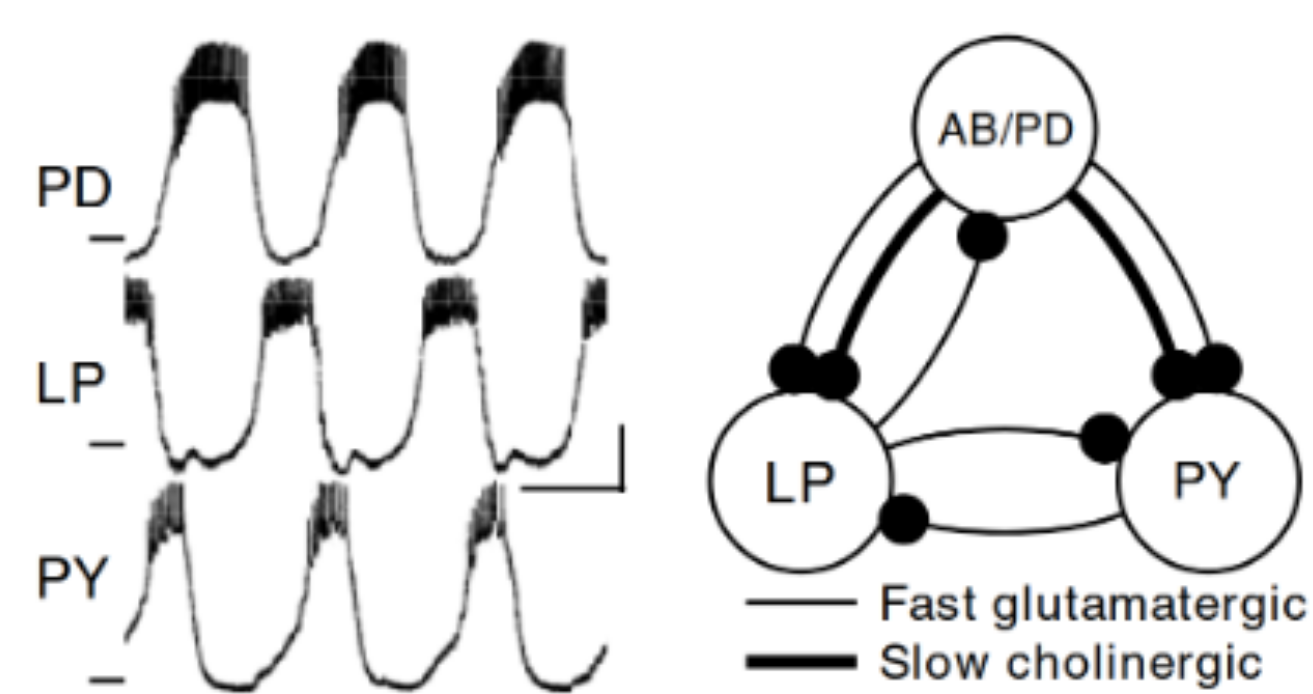
\includegraphics[width=0.66\linewidth]{../notebooks/network.png}
    \end{center}
    A 3-neuron Jaxley model (AB/PD, LP, PY) with \highlight{7 free synaptic
    conductances}:
    \vskip0.2cm
    {\small\begin{tabular}{ll}
      \toprule
      \textbf{Synapse} & \textbf{Type} \\
      \midrule
      AB/PD $\to$ LP (×2) & Glut + Chol \\
      AB/PD $\to$ PY (×2) & Glut + Chol \\
      LP $\to$ AB/PD & Glutamatergic \\
      LP $\to$ PY    & Glutamatergic \\
      PY $\to$ LP    & Glutamatergic \\
      \bottomrule
    \end{tabular}}
    \vskip0.2cm
    Parameters are searched in \textbf{log-space}: $\theta_i = \log_{10}(g_i)$,
    prior $\theta_i \sim \mathcal{U}(-5,\,1)\ \mu\text{S}$.
  \end{block}

  \begin{block}{Summary Statistics (9 features)}
    \small
    \begin{tabular}{cl}
      \toprule
      \textbf{\#} & \textbf{Feature} \\
      \midrule
      0   & Burst period (ms) \\
      1--3 & Duty cycle: AB/PD, LP, PY \\
      4--5 & Phase offset: LP, PY (re AB/PD) \\
      6--8 & Spikes/burst: AB/PD, LP, PY \\
      \bottomrule
    \end{tabular}
    \vskip0.3cm
    Phase offsets are \highlight{weighted 3$\times$} in the DE loss because
    they capture the triphasic coordination most sensitively.
    For non-bursting simulations, a NaN penalty of 10 is assigned.
  \end{block}

\end{column}

%% ── COLUMN 2 ───────────────────────────────────────────────────────────────
\begin{column}{0.36\paperwidth}

  \begin{block}{Methods}
    \begin{columns}[t]
      \begin{column}{0.47\linewidth}
        \textbf{\method{Differential Evolution (DE)}}\\[0.3cm]
        Gradient-free global optimiser (SciPy). Treats the simulator as a
        black box — no differentiability required.
        \vskip0.2cm
        \begin{itemize}
          \item Population size: 5, max 50 generations
          \item Loss: weighted fractional error on 9 features
          \item \highlight{Best result: loss = 0.0073}
        \end{itemize}
        \vskip0.3cm
        \textit{Why not gradient descent?}\\
        Spike counts and burst periods are \textbf{step functions} —
        gradients vanish. Raw voltage MSE is phase-sensitive and traps
        gradient descent in local minima (wrong phase, right period).
        DE sidesteps both problems.
      \end{column}
      \begin{column}{0.47\linewidth}
        \textbf{\method{SNPE (Sequential NPE)}}\\[0.3cm]
        Amortised posterior inference using neural density estimation (sbi,
        SNPE-C / NPE).
        \vskip0.2cm
        \begin{itemize}
          \item Prior: log-uniform over $\log_{10}(g)$
          \item 500 forward simulations
          \item Neural posterior: masked autoregressive flow
          \item 2\,000 posterior samples drawn
        \end{itemize}
        \vskip0.3cm
        SNPE returns a full \textbf{posterior distribution} over all 7
        conductances, directly quantifying degeneracy without any
        additional sampling cost.
      \end{column}
    \end{columns}
  \end{block}

  \begin{block}{Result 1: DE Fit — Observed vs.\ Simulated}
    \begin{center}
      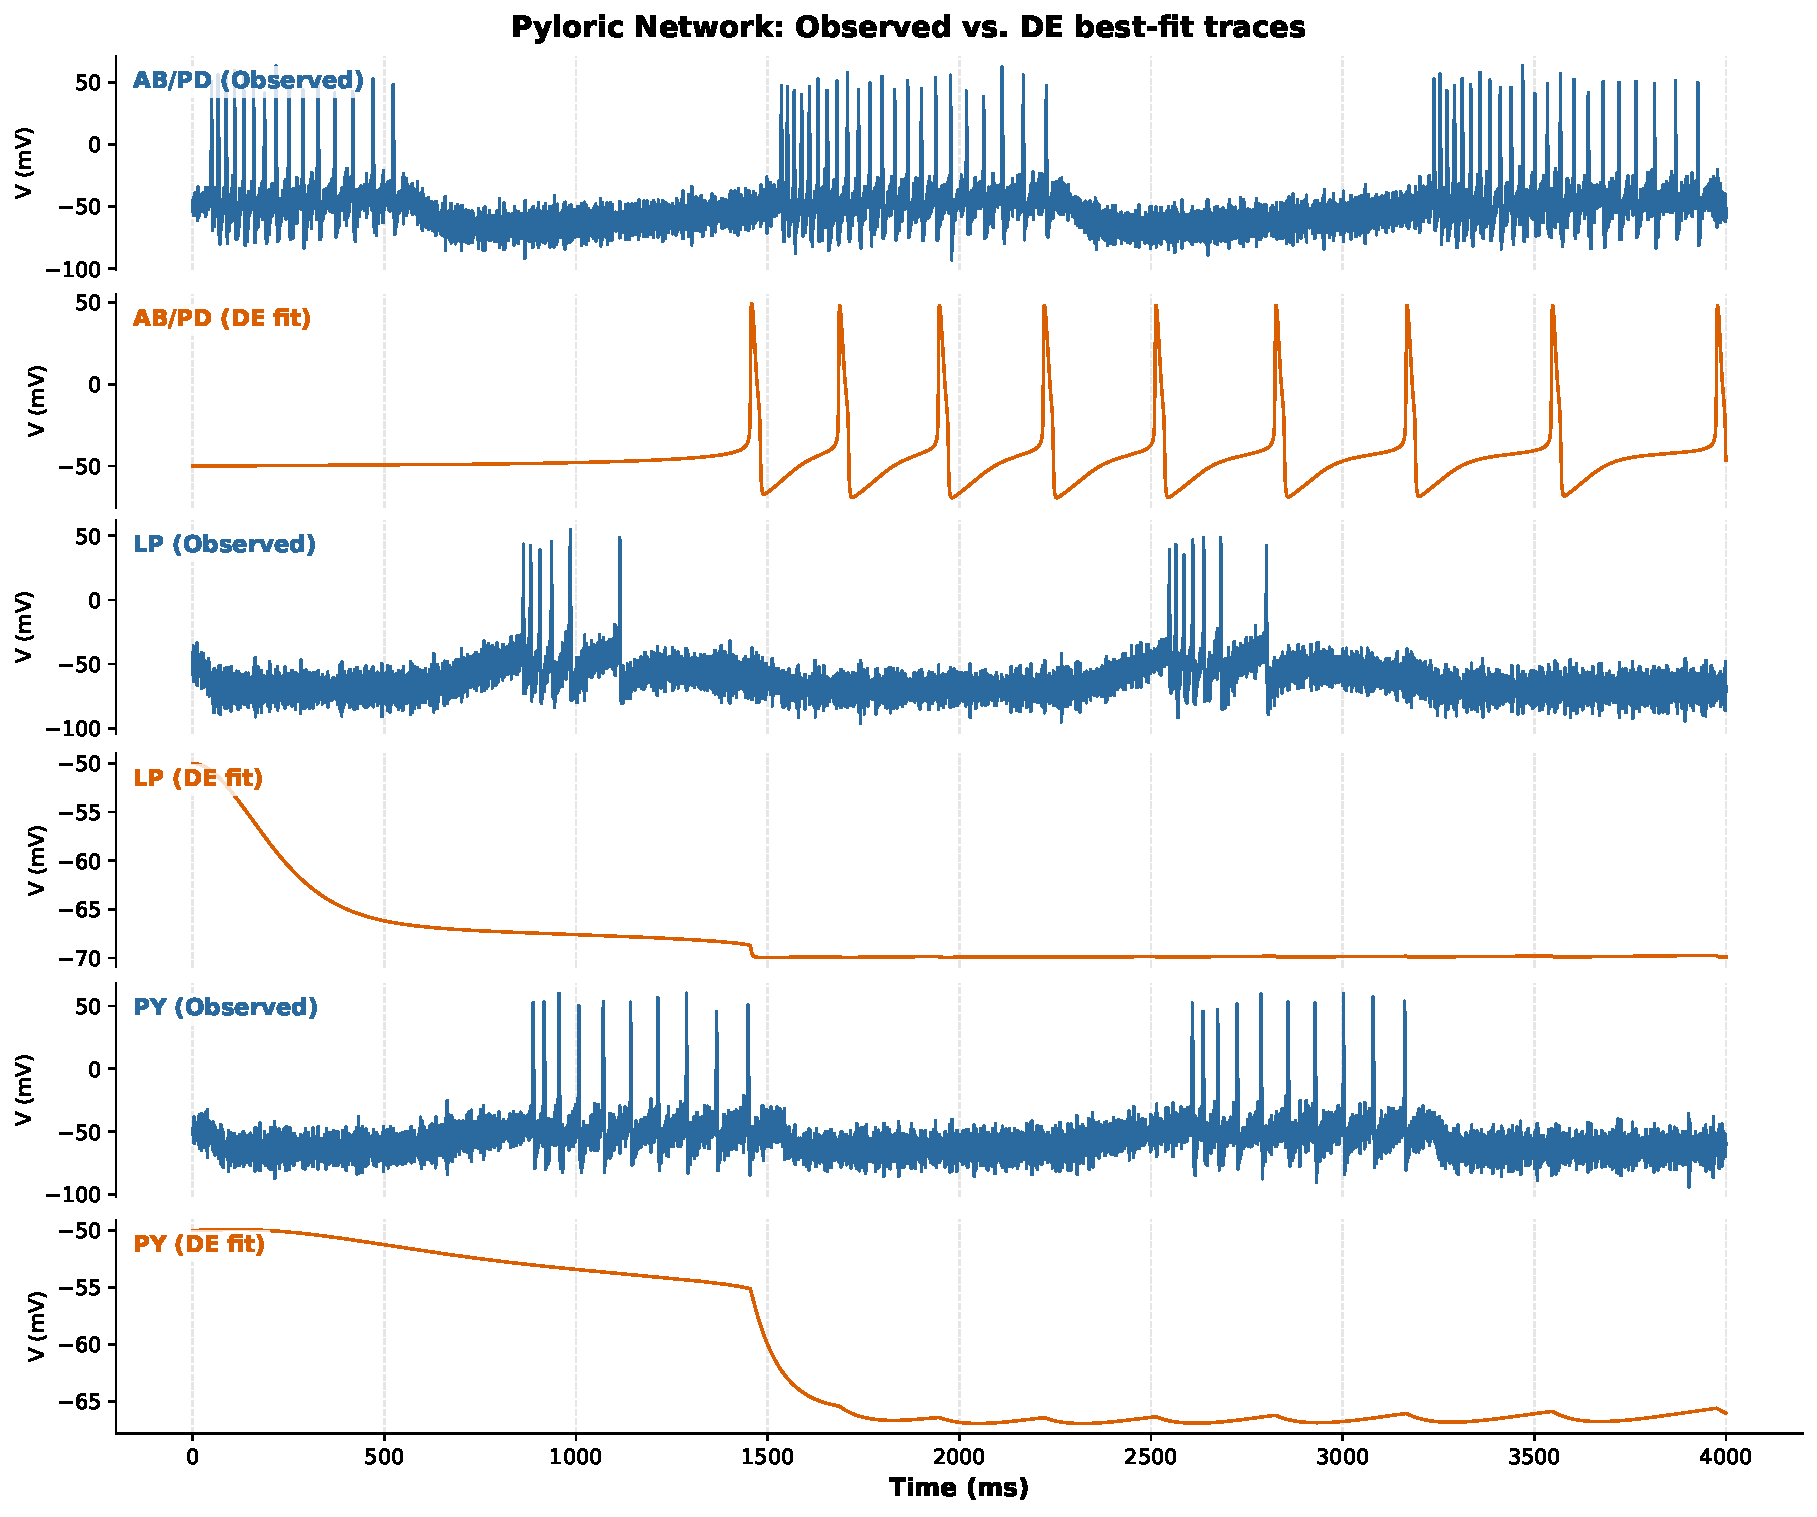
\includegraphics[width=0.80\linewidth]{../notebooks/fig_de_fit.pdf}
    \end{center}
    \small
    DE best-fit (orange) vs.\ observed (blue): period, duty cycles, phase
    offsets, and spike counts matched with \highlight{$\approx$7\% fractional
    error} across all 9 features.
  \end{block}

  \begin{block}{Result 2: Posterior Predictive Check}
    \begin{center}
      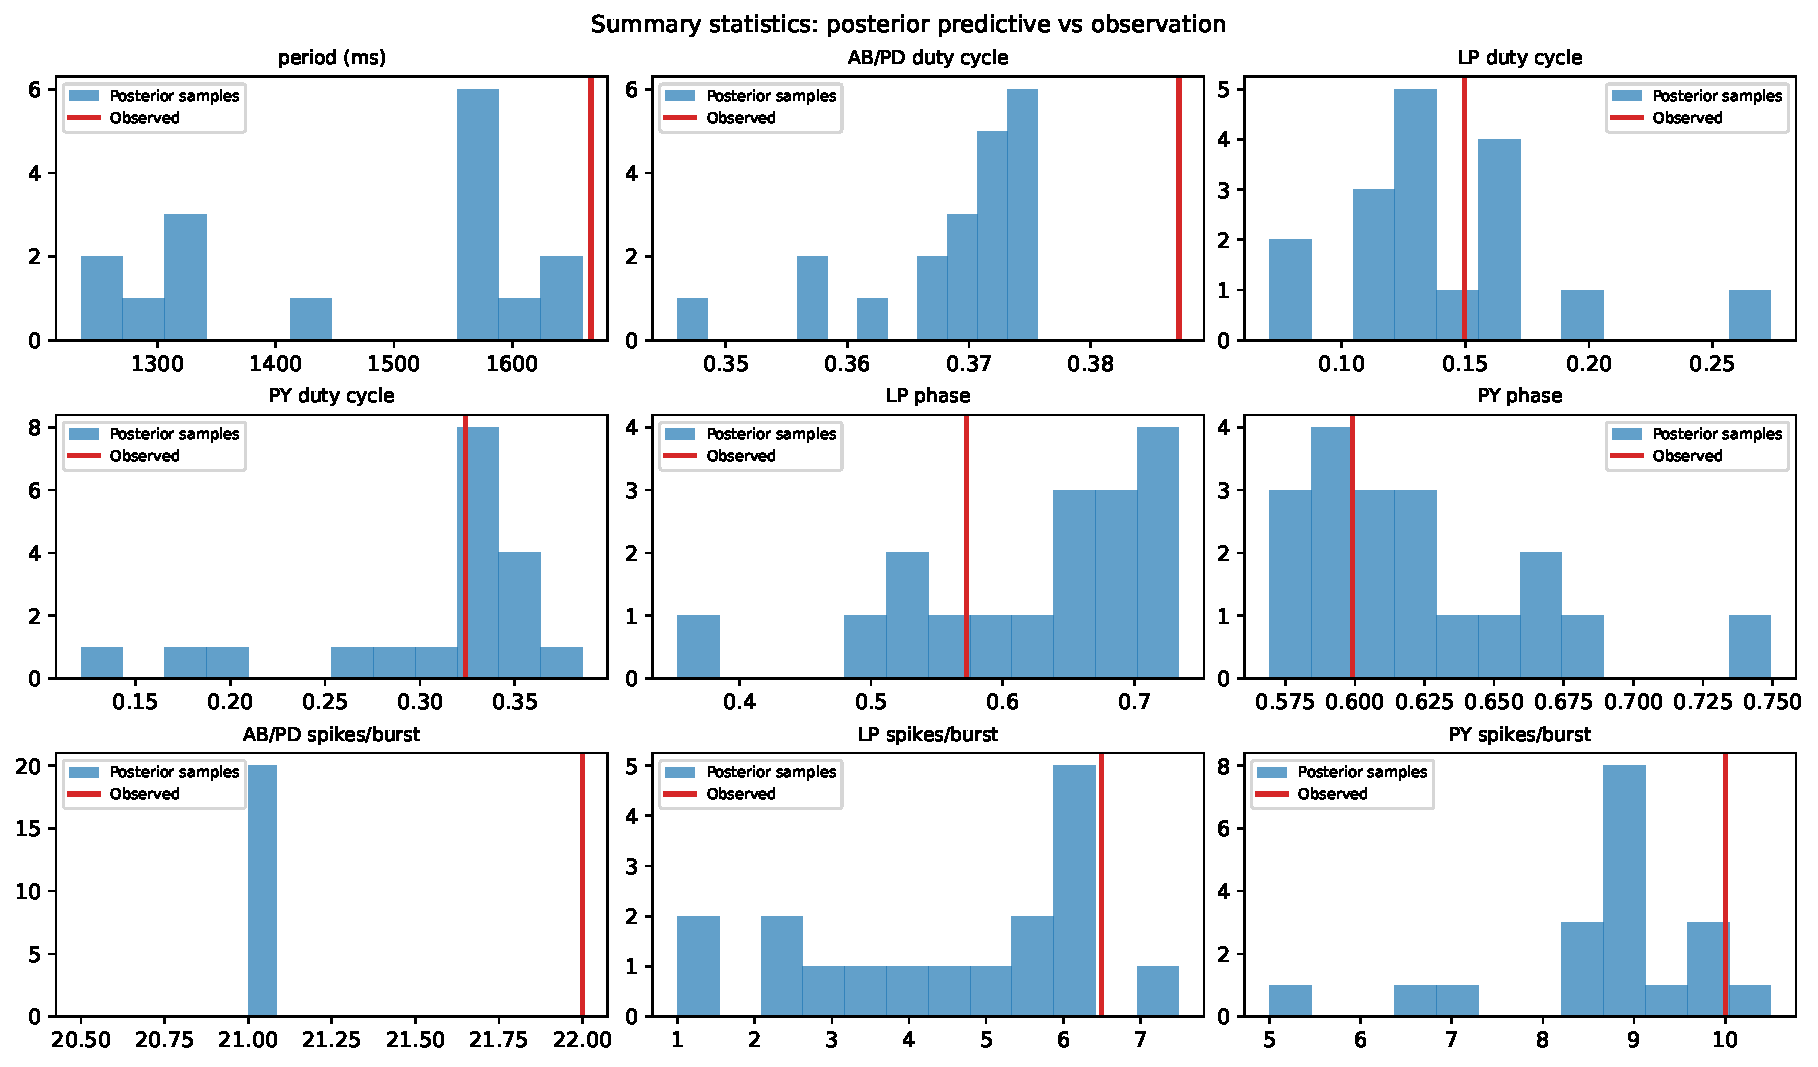
\includegraphics[width=0.76\linewidth]{../notebooks/fig_stats_comparison.pdf}
    \end{center}
    \small
    Histograms of summary statistics from 20 posterior samples (blue) vs.\
    the observed target value (red line). Statistics within the posterior
    predictive distribution confirm that the SNPE posterior captures
    the data-generating features.
  \end{block}

\end{column}

%% ── COLUMN 3 ───────────────────────────────────────────────────────────────
\begin{column}{0.31\paperwidth}

  \begin{block}{Result 3: Degeneracy — Posterior Trace Overlay}
    \begin{center}
      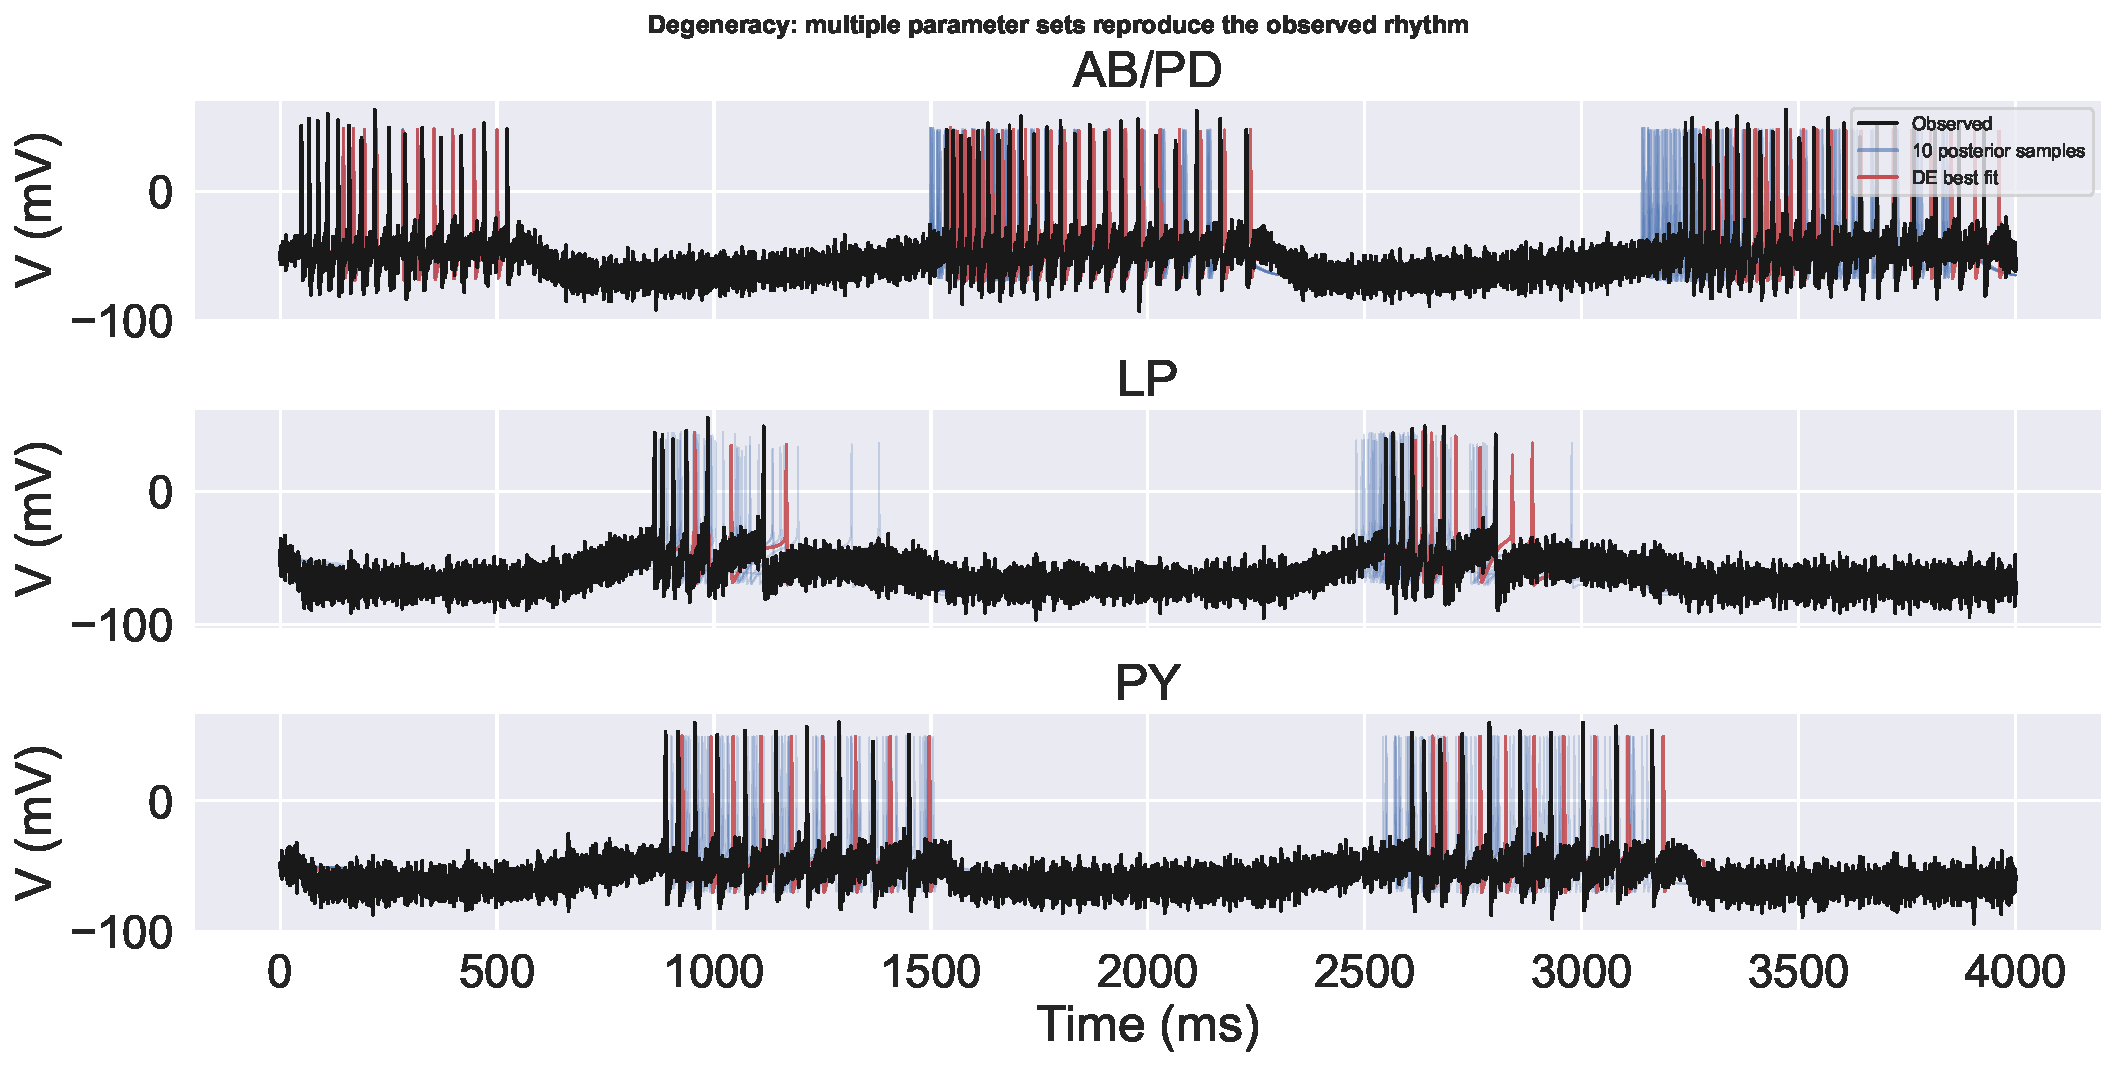
\includegraphics[width=0.78\linewidth]{../notebooks/fig_degeneracy_overlay.pdf}
    \end{center}
    \small
    Observed (black), 20 posterior samples (blue), DE best (red).
    All produce \highlight{functionally equivalent rhythms} — different
    conductances, indistinguishable behaviour.
  \end{block}

  \begin{block}{Result 4: Posterior over Conductances}
    \begin{center}
      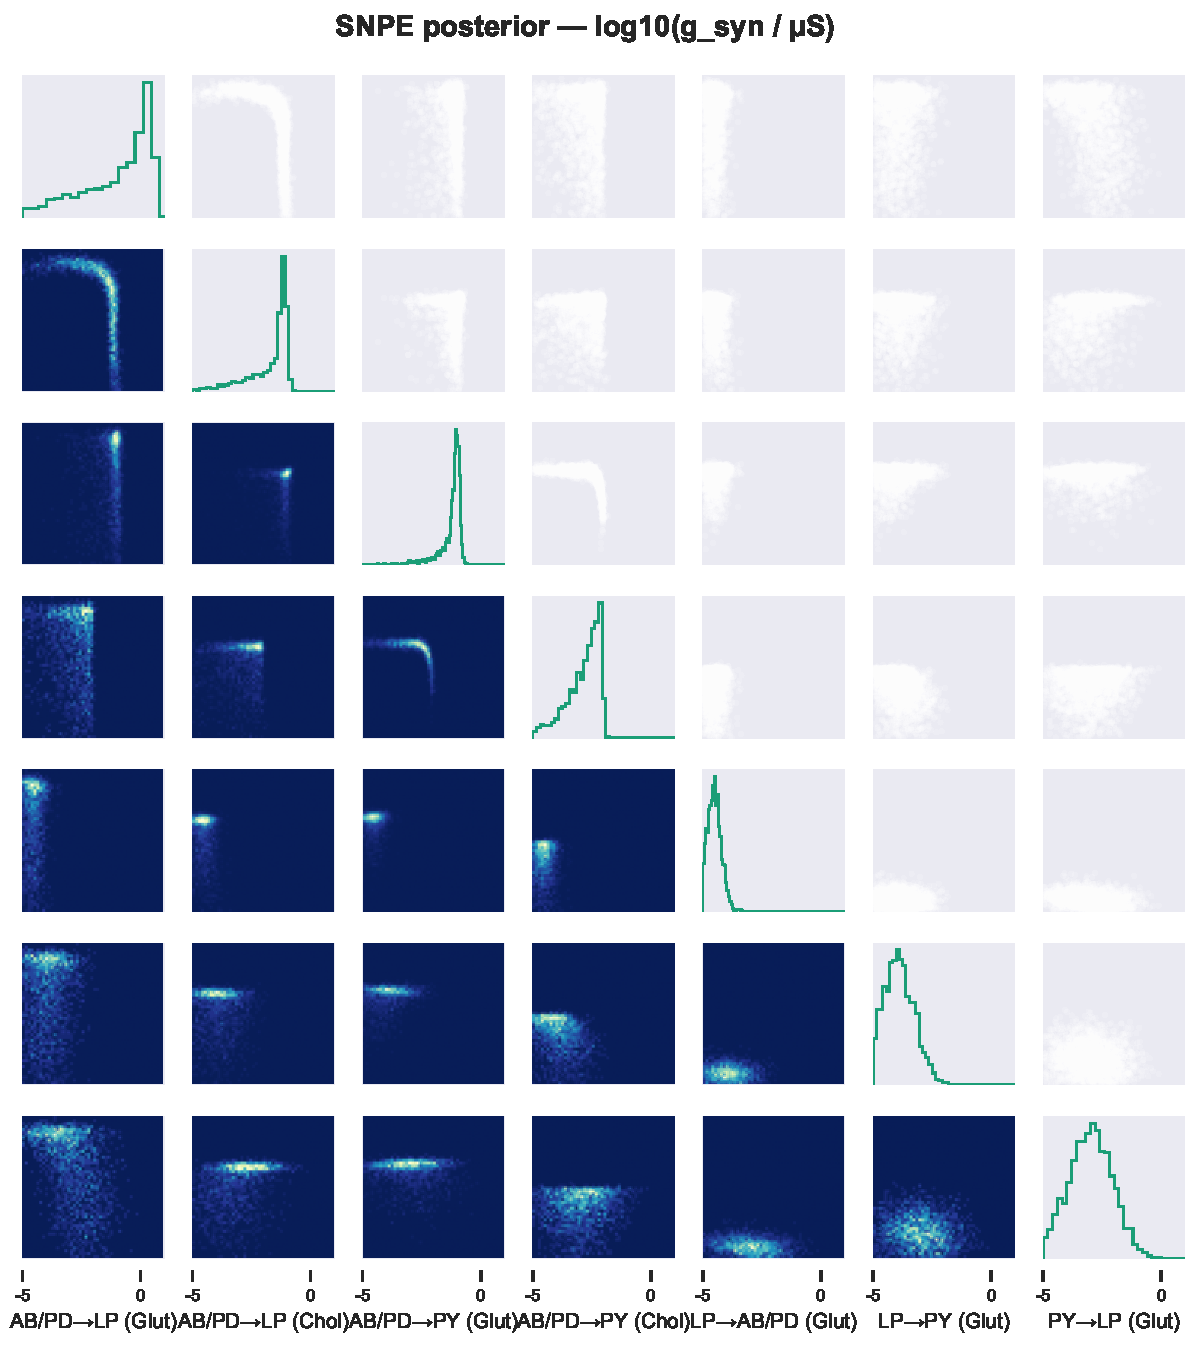
\includegraphics[width=0.70\linewidth]{../notebooks/fig_posterior_pairplot.pdf}
    \end{center}
    \small
    Pairplot of the SNPE posterior over all 7 log-conductances ($\log_{10}g$).
    Broad marginals and weak pairwise correlations indicate that the
    inverse problem is \highlight{underdetermined} — a wide range of
    conductance combinations fits the observation equally well.
  \end{block}

  \begin{alertblock}{Conclusions}
    \begin{enumerate}
      \item \textbf{DE recovers a good fit.}
            Loss of 0.0073 ($\approx$7\% fractional error) with a
            visually convincing trace match.
      \item \textbf{The posterior is broad.}
            SNPE reveals substantial posterior uncertainty, consistent
            with Prinz et al.\ (2004).
      \item \textbf{Degeneracy is real.}
            20 distinct posterior samples all produce valid triphasic
            rhythms — the recording cannot uniquely identify conductances.
      \item \textbf{Phase offsets are most informative.}
            The 3$\times$-weighted phase features dominate the DE loss
            and constrain the posterior most tightly.
    \end{enumerate}
  \end{alertblock}

\end{column}
\end{columns}

\end{frame}
\end{document}
